\documentclass{article}

\usepackage{tikz}
\usepackage{pdfpages}
\usepackage{parskip}
\usepackage{amsmath}
\usepackage[margin=.6in]{geometry}

\begin{document}
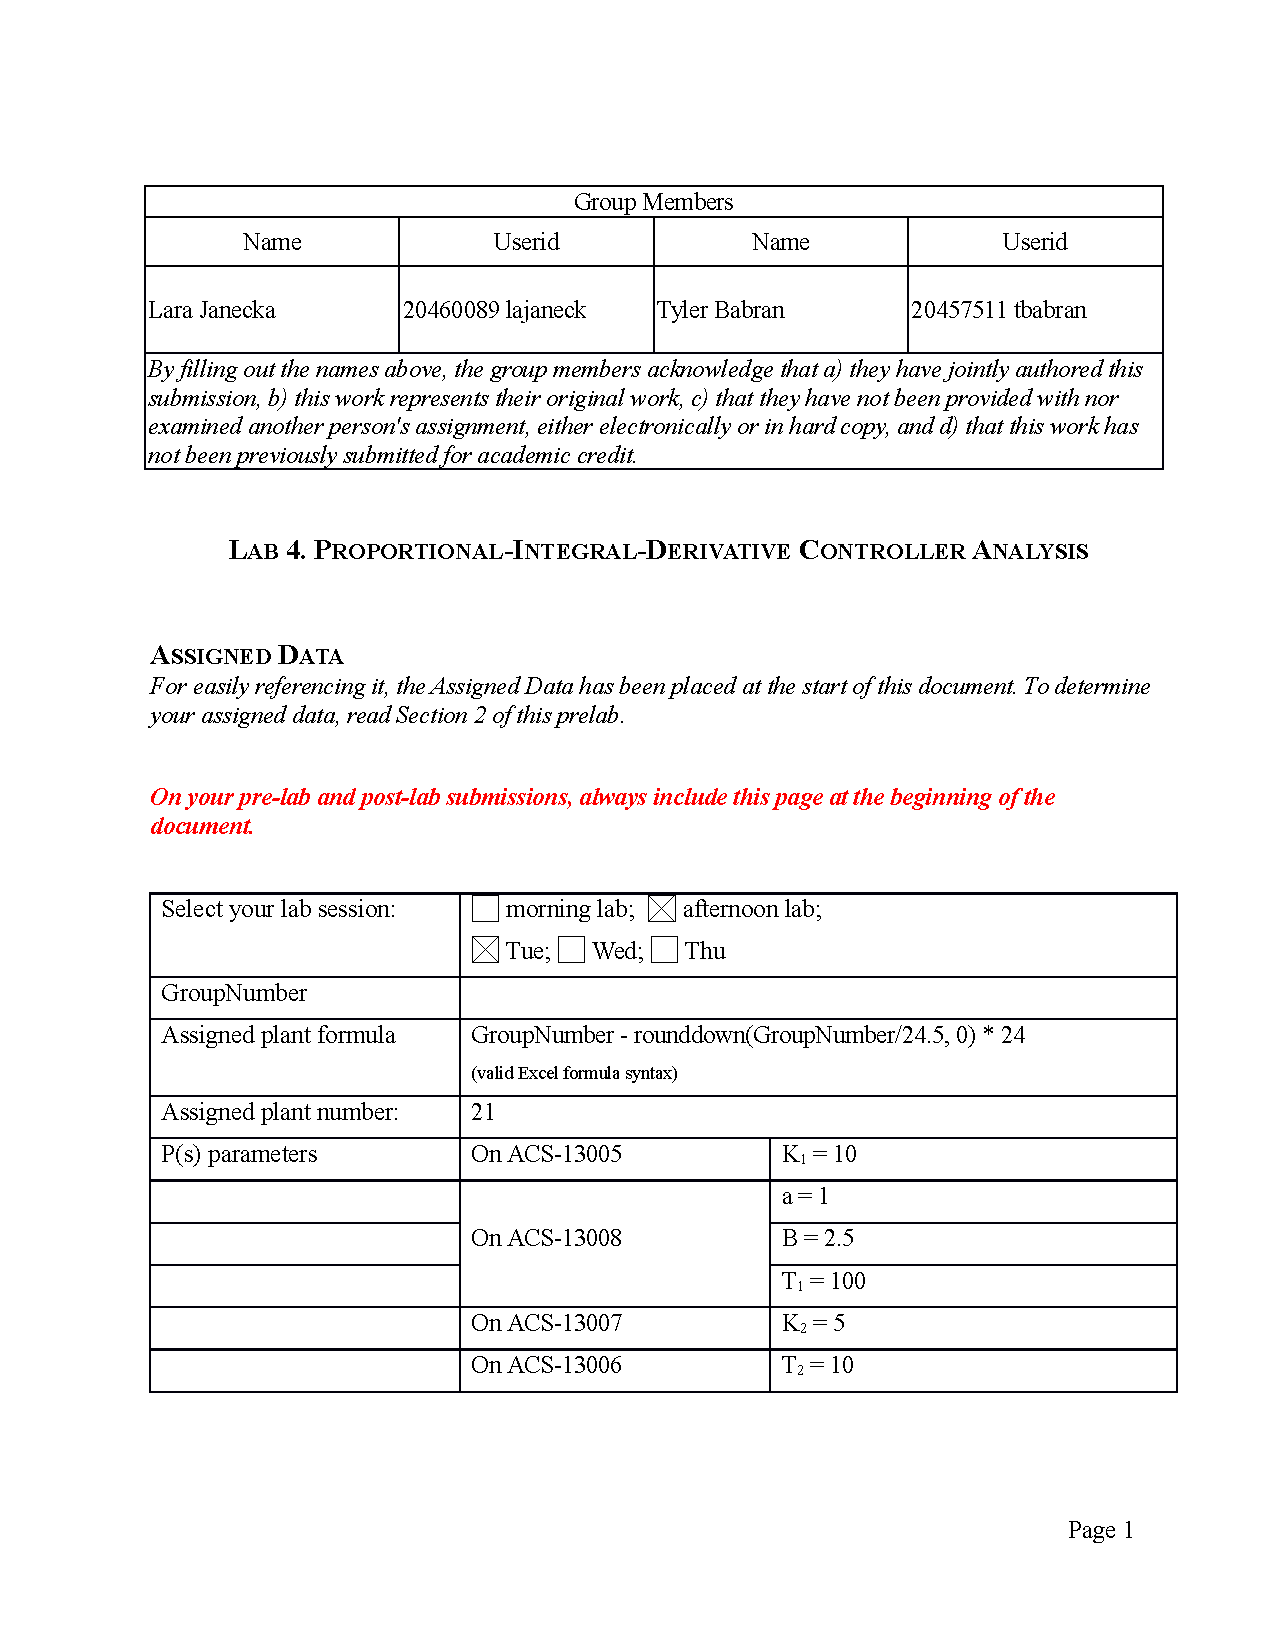
\includepdf[pages={1}]{page1.pdf}

\section*{5.1} % (fold)

\begin{table}[!htbp]
\centering
    \begin{tabular}{|c|c|c|c|}
        \hline
        &  $M_p$ & $y_{ss}$ & $T_p$ \\
        &  (V) & (s) & (s) \\
        \hline
        \textbf{Experimental} & 0.11 & 0.1 & 0.09\\
        \hline
        \textbf{Simulated} & 0.11 & 0.1 & 0.08\\
        \hline
        \textbf{Errors} & 0 & 0 & 0.18\\
        \hline
    \end{tabular}
    \caption{Plant verification results}
\end{table}


\begin{figure}[!htbp]
    \centering
    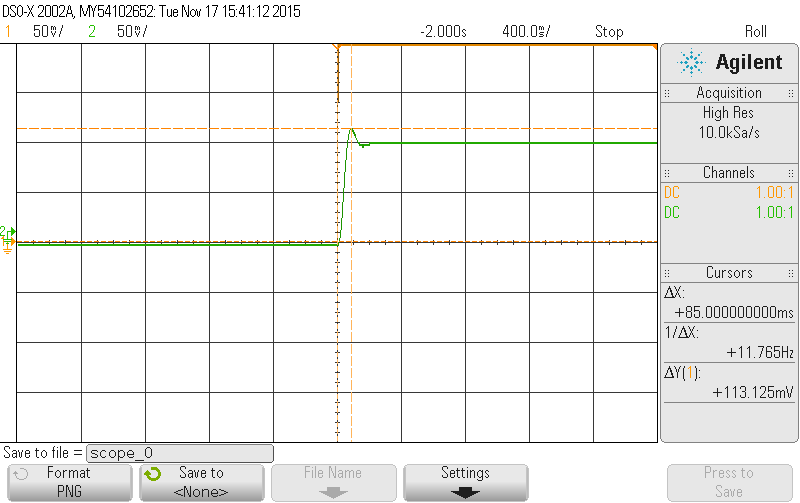
\includegraphics[width=0.95\textwidth]{5_1.png}
    \caption{Plant verification response}
\end{figure}
% section 5_1 (end)

\section*{5.2} % (fold)
\subsection*{a} % (fold)
The minimum value of $K_p$ to cause instability was 5.55. This was determined by slowly increasing the gain until the response stopped converging.
% subsection a (end)
\newpage
\subsection*{b} % (fold)
\begin{table}[!htbp]
\centering
    \begin{tabular}{|c|c|c|c|c|c|c|}
        \hline
        $K_p$ & $T_p$ & $M_p$ & $y_{ss}$ & OS & $e_{ss}$ & $T_s$2\% \\
        \hline
        & (s) & (V) & (V) & \% & \% & (s) \\
        \hline
        1 & 0.09 & 0.11 & 0.1 & 14 & 50 & 0.19\\
        \hline
        2 & 0.08 & 0.17 & 0.13 & 33.08 & 35 & 0.23\\
        \hline
        3 & 0.07 & 0.21 & 0.14 & 44.44 & 28 & 0.36\\
        \hline
        4 & 0.055 & 0.24 & 0.16 & 54.84 & 22.5 & 0.4\\
        \hline
    \end{tabular}
    \caption{Measurements of P-controlled system}
\end{table}
% subsection b (end)

\subsection*{c} % (fold)
As $K_p$ increases the first peak occurs faster and peaks higher. This results in an increase in overshoot. The steady-state error decreases at the cost of an increased settling time. This can also be seen in the increasing settling value.
% subsection c (end)

\subsection*{d} % (fold)
\begin{figure}[!htbp]
    \centering
    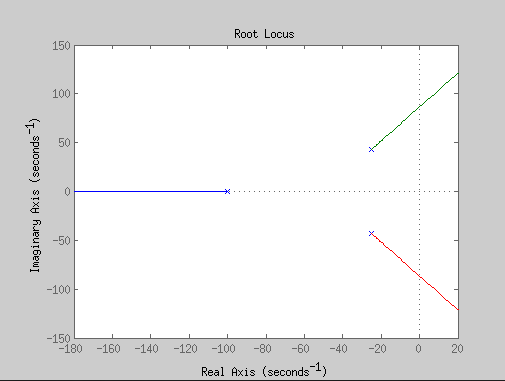
\includegraphics[width=0.95\textwidth]{5_2_locus.png}
    \caption{Root locus of system under proportional control}
\end{figure}
% subsection d (end)

\subsection*{e} % (fold)
The height of the first peak is proportional to overshoot which is proportional to the angle from the origin to the poles. As can be seen on the root locus as $K_p$ increases the angle of the poles increases which is why the height of the first peak and overshoot increase with $K_p$. The time to the first peak is inversely proportional the imaginary part of the pole. The root locus shows as $K_p$ increases the imaginary part of the poles increases which corresponds to our time to first peak decreasing. The settling time is inversely proportional to the real part of the poles and as $K_p$ increases the real part of the poles decreases causing the settling time to increase. The settling value increases since it is directly proportional to the gain which is $K_p$. The error is the difference between the input and steady-state value and we can see our steady-state value increasing towards the input as $K_p$ increases so the error decrease with it. We can ignore the pole traveling along the real axis as it gets farther away from the imaginary axis allowing the other poles to dominate it.
% subsection e (end)

\subsection*{f} % (fold)
You can reduce your steady-state error by increasing $K_p$ until steady-state value reaches the input value provided that it does not cause the system to become unstable. For our system we approach 8 and in a general case it can approach the value of $K_p$ where the root locus crosses the imaginary axis.
% subsection f (end)
% section 5_2 (end)

\section*{5.3} % (fold)
\subsection*{a} % (fold)
\begin{table}[!htbp]
\centering
    \begin{tabular}{|c|c|c|c|c|c|c|}
        \hline
        $K_i$ & $T_p$ & $M_p$ & $y_{ss}$ & OS & $e_{ss}$ & $T_s$2\% \\
        \hline
        30 & 0.1 & 0.24 & 0.2 & 21.5 & 0 & 0.3\\
        \hline
        40 & 0.1 & 0.27 & 0.2 & 35 & 0 & 0.5\\
        \hline
        50 & 0.09 & 0.3 & 0.2 & 50 & 0 & 0.73\\
        \hline
        60 & 0.085 & 0.33 & 0.2 & 65 & 0 & 1.08\\
        \hline
    \end{tabular}
    \caption{Measurements of PI-controlled system}
\end{table}
\newpage
\begin{figure}[!htbp]
    \centering
    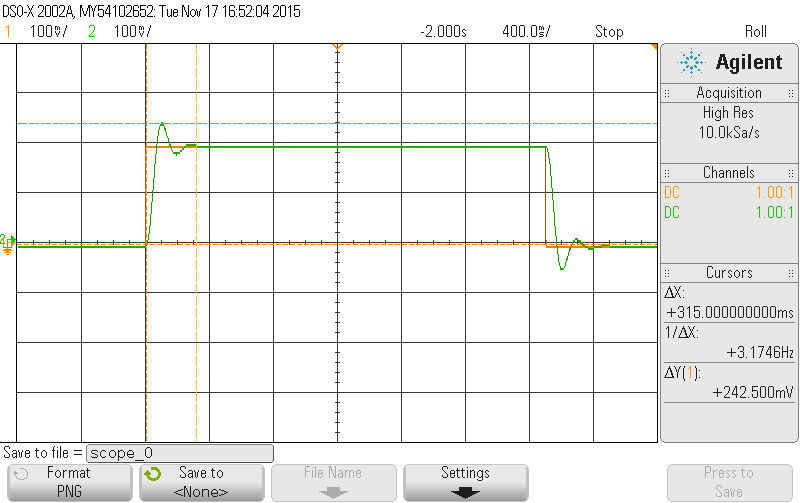
\includegraphics[width=0.95\textwidth]{5_3.png}
    \caption{P-I controlled system response}
\end{figure}
% subsection a (end)

\subsection*{b} % (fold)
As $K_i$ increased the height of the first peak and the overshoot increased. The steady-state value stayed equal to the input value resulting in no error regardless of $K_i$. The time to first peak plateaued then decreased and the settling time increased as $K_i$ increased.
% subsection b (end)
\newpage
\subsection*{c} % (fold)
\begin{figure}[!htbp]
    \centering
    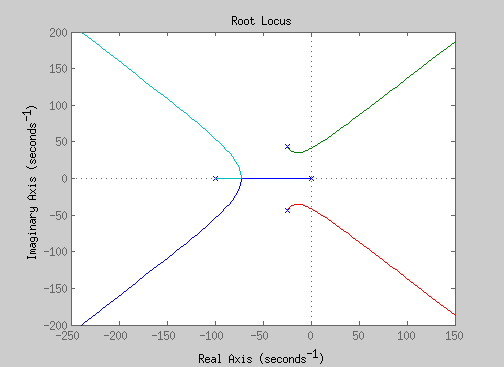
\includegraphics[width=0.95\textwidth]{5_3_locus.png}
    \caption{Root locus of P-I controlled system}
\end{figure}
% subsection c (end)

\subsection*{d} % (fold)
The height of the first peak and overshoot are is proportional to the angle of the poles. As $K_i$ increases the angle of the poles increases which is why the height of the first peak and overshoot increase with $K_i$. The settling value increases since it is directly proportional to the gain which is $K_p$ and this did not change. Similarly the error did not change. The time to the first peak is inversely proportional the imaginary part of the pole. The root locus shows as $K_i$ increases the imaginary part of the poles bowls for a short bit then increases which corresponds to our time to first peak recordings. The settling time is inversely proportional to the real part of the poles and as $K_i$ increases the real part of the poles decreases causing the settling time to increase. We can ignore the two branches of the root locus heading to infinity as these are quickly dominated by the other two branches.

% subsection d (end)
% section 5_3 (end)
\newpage
\section*{5.4} % (fold)

\subsection*{a} % (fold)
\begin{table}[!htbp]
\centering
    \begin{tabular}{|c|c|c|c|c|c|c|}
        \hline
        $K_d$ & $T_p$ & $M_p$ & $y_{ss}$ & OS & $e_{ss}$ & $T_s$2\% \\
        \hline
        0 & 0.09 & 0.1 & 0.1 & 0  & 50 & 0.24\\
        \hline
        0.33 & 0.05 & 0.1 & 0.1 & 0  & 50 & 0.1\\
        \hline
        0.66 & 0.14 & 0.1 & 0.1 & 0  & 50 & 0.14\\
        \hline
        0.1 & 0.18 & 0.1 & 0.1 & 0  & 50 & 0.18\\
        \hline
    \end{tabular}
    \caption{Measurements of PD-controlled system}
\end{table}

\begin{figure}[!htbp]
    \centering
    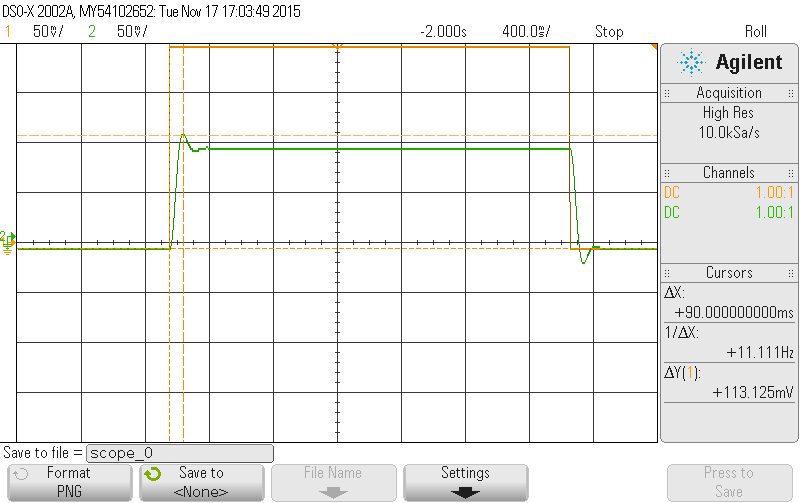
\includegraphics[width=0.95\textwidth]{5_4.png}
    \caption{P-D controlled system response}
\end{figure}
% subsection a (end)
\subsection*{b} % (fold)
As $K_d$ increases the time to first peak dips slightly then increases. The value of the first peak slightly decreases and the settling value remains roughly the same. The overshoot also remained the same. The steady-state error remains roughly the same and the settling time dips and then increases.

% subsection b (end)
\newpage
\subsection*{c} % (fold)
\begin{figure}[!htbp]
    \centering
    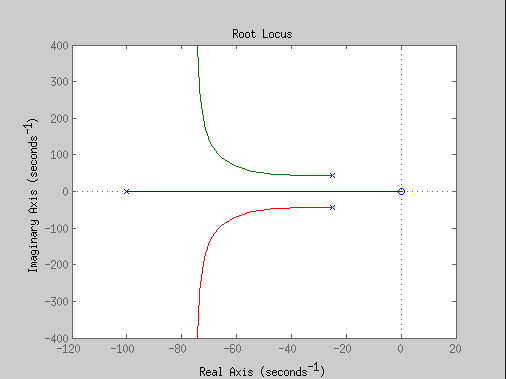
\includegraphics[width=0.95\textwidth]{5_4_locus.png}
    \caption{Root locus of P-D controlled system}
\end{figure}
% subsection c (end)
\subsection*{d} % (fold)
The time to the first peak dips while the imaginary poles are dominating due to their imaginary parts increasing (it has an inverse relationship), but begins to rise as the real pole starts dominating. The same can be said for the settling time which is inversely proportional to the real part of the poles causing it to decrease while the complex poles dominate and increase when the real pole starts dominating. The overshoot is zero for all values due to the angle of the poles being very small while the complex poles dominated (likely due to rounding errors when reading these values) and then dropping to zero when the real pole dominates. This same logic applies to why the height of the first peak remains roughly the same. The settling value is proportional to $K_p$ which remained constant keeping it constant. This also resulted in the steady-state error remaining constant as neither the input nor steady-state value changed.
% subsection d (end)
% section 5_4 (end)
\newpage
\section*{5.5} % (fold)
\subsection*{a} % (fold)
\begin{table}[!htbp]
\centering
    \begin{tabular}{|c|c|c|c|c|c|c|c|c|}
        \hline
        $K_p$ & $K_i$ & $K_d$ & $T_p$ & $M_p$ & $y_{ss}$ & OS & $e_{ss}$ & $T_s$2\% \\
        \hline
        1 & 25.2 & 0.02 & 0.13 & 0.2 & 0.2 & 0 & 0 & 0.13\\
        \hline
    \end{tabular}
    \caption{PID controlled system}
\end{table}
% subsection a (end)
\subsection*{b} % (fold)
Increasing $K_i$ by large amounts eliminated the steady-state error, but increased the overshoot. Adding in $K_d$ eliminated the overshoot without increasing the settling time excessively. Together they produced a stable system that responded quickly.

% subsection b (end)
\subsection*{c} % (fold)
To improve the steady-state performance of our system you only need to add integral action.

% subsection c (end)


% section 5_5 (end)


\end{document}
